%%%%%%%%%%%%%%%%%%%%%%%%%%%%%%%%%%%%%%%%%%%%%%%%%%%%%%%%%%%%%%%%%%%%%%
%%                     And
%%%%%%%%%%%%%%%%%%%%%%%%%%%%%%%%%%%%%%%%%%%%%%%%%%%%%%%%%%%%%%%%%%%%%%
%\color{blue}
\subsection{Glyph: \glyph{And}}\label{sec:and}

The glyph \glyph{and} is used to denote that all the \glyph{EPNs} linked as input are necessary to produce the output influence.  

\begin{glyphDescription}
 \glyphSboTerm SBO:0000173 ! and.
 \glyphOrigin One interactor (section~\ref{sec:interactors}) or logical operator (section~\ref{sec:logic}).
 \glyphTarget  One modulation (section~\ref{sec:modulation}), stimulation (section~\ref{sec:stimulation}), inhibition (section~\ref{sec:inhibition}), necessary  stimulation (section~\ref{sec:necessaryStimulation}), or absolute inhibition (section~\ref{sec:absoluteInhibition}) arc.
 \glyphNode \glyph{Not} is represented by a circle carrying the word  ``AND''.
\end{glyphDescription}

\begin{figure}[H]
  \centering
  \includegraphics[scale = 0.5]{images/and}
  \caption{The \PD glyph for \glyph{and}. Only two inputs are represented, but more would be allowed.}
  \label{fig:and}
\end{figure}


% The following diagrams illustrate the dephosphorylation of the MAP inase ERK by the protein phosphatase 2A and the STriatal Enriched Phosphatase, in ST (left) and ER (right). 
% 
% \begin{center}
% \scalebox{0.5}{\includegraphics{images/stimulation-example1}}
% \end{center}
\normalcolor
